\documentclass[authoryear,preprint,review,10pt]{elsarticle}
\usepackage{amssymb,amsthm,amsmath,setspace,paralist}
\usepackage{url}
\usepackage[usenames,dvipsnames]{color}
\usepackage{lineno}
%\usepackage[labelfont=bf,format=hang,textfont=it]{caption}
\usepackage{graphicx}
\usepackage{microtype}
\usepackage[letterpaper,text={15cm,23cm}]{geometry}
\usepackage{natbib}
\usepackage{hyperref}
\usepackage{subfig}
%\usepackage{times} % Time New Roman

\bibliographystyle{model5-names} 

%% for internal use
\newcommand{\fixme}[1]{\emph{\marginpar{FIXME} (#1)}}
\newcommand{\readme}[1]{\emph{\marginpar{README} (#1)}}

\newcommand{\degree}{\ensuremath{^\circ}}

\definecolor{Red}{rgb}{0.5,0,0}
\definecolor{Blue}{rgb}{0,0,0.5}
\hypersetup{%
  pdftitle = {Near real-time disturbance detection in terrestrial ecosystems using satellite image time series: Drought detection in Somalia},
  pdfsubject = {remote sensing, monitoring},
  pdfkeywords = {early warning, real-time monitoring, global change, disturbance, time series, remote sensing, vegetation and climate dynamics},
  pdfauthor = {Jan Verbesselt, Achim Zeileis, Martin Herold},
  %% change colorlinks to false for pretty printing
  colorlinks = {true},
  linkcolor = {Blue},
  citecolor = {Blue},
  urlcolor = {Red},
  hyperindex = {true},
  linktocpage = {true},
}

\begin{document}
%\linenumbers

\begin{frontmatter}

    \title
    {
Near real-time disturbance detection in terrestrial ecosystems using satellite image time series: \\ Drought detection in Somalia
    }
    \author[WUR]{Jan Verbesselt\corref{cor}}
    \ead{Jan.Verbesselt@wur.nl}
    \author[UIBK]{Achim Zeileis}
    \ead{Achim.Zeileis@R-project.org}
    \author[WUR]{Martin Herold}
    \ead{Martin.Herold@wur.nl}
    \cortext[cor]{Corresponding author.}
    \address[WUR]{Remote Sensing Team, Wageningen University, \\
           Droevendaalsesteeg 3, Wageningen 6708 PB, The Netherlands \\
           \emph{Ph}: + 31 317 48 52 68; \emph{Fax}: +31 317 419000}
    \address[UIBK]{Department of Statistics, Universit\"at Innsbruck \\
           Universit\"atsstr.~15, A-6020 Innsbruck, Austria}

%http://www.fao.org/giews/pricetool2/
\begin{abstract}
Near real-time monitoring of ecosystem disturbances is critical for addressing impacts on carbon dynamics, biodiversity, and socio-ecological processes. Satellite remote sensing enables cost-effective and accurate monitoring at frequent time steps over large areas. Yet, generic methods to detect disturbances within newly captured satellite images are lacking. 
We propose a generic time series based disturbance detection approach by modelling \emph{stable} historical behaviour to enable detection of \emph{abnormal} changes within newly acquired remotely sensed data.
Satellite image time series of vegetation greenness provide a global record of terrestrial vegetation productivity over the past decades. Here, we assess and demonstrate the method by applying it to (1)~simulated time series of vegetation greenness data from satellite data, (2)~real satellite greenness image time series between February 2000 and July 2011 covering Somalia to  detect drought related vegetation disturbances.
First, simulation results illustrate that disturbances are successfully detected in near real-time while being robust for seasonality and noise. Second, major drought related disturbance corresponding with most drought stressed regions in Somalia are detected from mid 2010 onwards and illustrate the proof-of-concept of the method. The method can analyse in-situ or satellite data time series of biophysical indicators from local to global scale since it is fast, does not depend on thresholds or definitions and does not require time series gap filling. While the data and methods used are appropriate for proof-of-concept development for global scale disturbance monitoring, specific operational applications (e.g., drought or deforestation monitoring) mandates integration within an early warning framework (e.g.\ \url{www.fews.net} and the FAO Global Information and Early Warning System).
\end{abstract}


\begin{keyword}
Early warning \sep real-time monitoring \sep global change \sep disturbance \sep time series \sep remote sensing \sep vegetation phenology \sep climate dynamics
\end{keyword}

\end{frontmatter}

%Time series of satellite vegetation greenness provide a measure for terrestrial vegetation productivity dynamics over the last decades covering the whole world. 

%\newpage

\section{Introduction}

%Real-time disturbance detection is critical for tracking human- and climate- induced changes promptly \citep{Asner:2011fa}. Such information is needed for signalling abnormal developments, quickly raising awareness and reducing negative impacts to natural resources, humans, and infrastructure. Key to approaches looking at disturbances is that many recent change events occur worldwide at unknown locations.

Real-time disturbance detection is critical for signalling abnormal developments, quickly raising awareness and reducing negative impacts to natural resources, humans, and infrastructure. A disturbance can be defined as a relatively discrete event occurring over a short time period that disrupts the structure of an ecosystem, community, or population, and changes resource availability or the physical environment \citep{Pickett:1986td}. Disturbances alter the system state and the trajectory of an ecosystem, and therefore are the key drivers of spatial and temporal heterogeneity \citep{Turner:2010wo}. Abiotic (e.g. fires, windstorms) and biotic (e.g. pest, pathogens) ecosystem disturbances can contribute to the current rise of carbon dioxide ($CO_2$) levels in the atmosphere due to the emission of $CO_2$ from terrestrial biomass loss \citep{Potter2003,Schimel:2001vi}. 
Many recent disturbances occur worldwide at unknown locations. In this sense, remote sensing tools can be in the first instance used to alter for abrupt changes occurring in near real-time. For example, deviations from average land surface phenology pattern over multiple years, defined as the seasonal variation in vegetated land surface from satellite sensors \citep{White2009}, can indicate deforestation events \citep{Asner:2011fa}, forest health issues (e.g.\ tree mortality) \citep{Hargrove2009, Stone2008, Verbesselt2009}, drought and climate anomalies \citep{Funk:2009vf,Vrieling:2011da}.

% satellite data and vegetation indices
Satellite sensors are well-suited to provide consistent and frequent measurements over large areas which is appropriate for capturing the effects of many processes that cause disturbances, including physical (e.g.\ droughts, fires, floods), biogenic (e.g.\ herbivorous insects and pathogens) and anthropogenic (e.g.\ deforestation, urbanisation, farming) disturbances \citep{Jin2005, Potter2003}. A common way to derive indicators of ecosystem dynamics is the use of spectral vegetation indices related to the photosynthetic capacity of vegetation canopies such as the Normalised Difference Vegetation Index (NDVI) \citep[][]{Myneni1995, Pettorelli:2005ed, Potter2003}.  Although NDVI might be affected by soil background and a saturation effect at high biomass levels, it captures seasonal and inter-annual changes in vegetation status \citep{Huete2002,Myneni:1997ur}. 

Ecosystem changes commonly observed with remote sensing approaches can be divided into three categories: 
(1)~\emph{seasonal or cyclic change}, for example driven by annual temperature and rainfall interactions impacting plant phenology resulting in distinct intra-annual patterns for different vegetation types; 
(2)~\emph{gradual trend change} such as trends in mean annual rainfall or gradual change in land management (e.g., long term drought, forest regrowth after fire) that result in changes over several years; and 
(3)~\emph{abrupt trend change}, caused by events from human activities (e.g., deforestation) or natural causes (e.g., wind throw or an extreme drought event) that change land cover over short time frames (e.g. weeks or months) 
\citep{Beurs2005a,Verbesselt2009a,Verbesselt:2010wo}. 

% problem statement
Detecting changes within time series is the first step towards understanding the acting processes and drivers (e.g.\ natural or anthropogenic). Estimating change from remotely sensed data series however is not straightforward, since time series contain a combination of seasonal, gradual and abrupt ecosystem changes occurring in parallel, in addition to noise that originates from the sensing environment (e.g., view angle), remnant geometric errors, atmospheric scatter and cloud effects \citep{Beurs2005a, Roy2002, Wolfe1998}. 

The ability of any system to detect ecosystem disturbances depends on its capacity to differentiate the normal phenological cycle for an ecosystem from abnormal change. Several near real-time change detection methods utilising satellite data are available \citep{Jiang:2010ko, Verdin:2005by, White2006} but methods can be improved upon to detect disturbances in near real-time by utilising the full temporal detail of the data time series. Three major challenges remain;
% changes at the end of a time series -(what is normal and what is abnormal can maybe be mentioned above?)
First, it is crucial to be able to detect disturbances within newly captured satellite images to enable a rapid response or early warning. In previous work, we proposed an approach,  BFAST (Break detection For Additive Season and Trend), for change detection within seasonal time series \citep{deJong:wo, Verbesselt2009a,Verbesselt:2010wo}.
BFAST detects and characterises trend and seasonal changes within historical time series but the method is not developed to detect disturbances in recently acquired data. Methods to detect changes in near real-time, also referred to as monitoring techniques, have been suggested in the statistics and econometrics literature to assess the stability of linear regression models \citep{Chu1996}, e.g., for investigating exchange rate dynamics \citep{Zeileis:2010tt}. However, these methods have not been optimised for real-time disturbance detection of terrestrial ecosystems using remotely sensed time series data.

% threshold independent
Second, change detection techniques for global disturbance monitoring need to be independent of vegetation-specific thresholds while being robust against the inherent noise and seasonality captured within time series.
Most change detection methods require user designation of a threshold or change type definition separating real change from spectral changes caused by variability in illumination, seasonality, or atmospheric scattering \citep{Lu2004, Potter2003, Hayes2007}.  \citet{White2006} presented a method for real-time monitoring but it requires a region-specific threshold for detecting change. The determination of thresholds adds significant cost to efforts expanding change detection across regions or becomes complex when the regions are changing. A historical analysis using archived satellite data is needed to model normal, expected behaviour against which abnormal behaviour, i.e.\ disturbance, in the near future can be described \citep{Hargrove2009}. There is a critical need to enable analysis of time series independent of specific thresholds or definitions to detect disturbances.

% missing data: avoid smoothing and interpolation
Third, change detection methods need to deal with missing data (e.g., clouds or sensor defects) in time series data.
Existing change detection methods smooth or fill gaps \citep{Jonsson2002, Roerink2000, Julien2010} when dealing with noisy times series of remotely sensed data. For a given date, these methods typically require looking both backwards and forwards in time, negating use in real-time or forecast applications \citep{White2006}.  Furthermore, gap filling techniques model data based on assumptions of normal data variation which inhibits the detection of disturbances \citep{Samanta:2011hp}. Hence, methods able to analyse and detect changes in non-gap-filled time series are urgently needed for global change monitoring.

We propose a multi-purpose approach for near real-time disturbance detection using time series data that does not require specific thresholds and deals with missing data. The following major research questions are answered in this paper: \\
(1)~Can a period, representing stable (i.e.\ normal) historical data variation representing both seasonal and gradual changes, be identified within a time series?\\
(2)~Is the model representing a \emph{normal} historical data variation able to reliably and quickly differentiate between normal and \emph{abnormal} changes (i.e.\ disturbances) within newly incoming observations (i.e. near real-time)?

We assess this approach for different ecosystems by simulating NDVI time series with varying amounts of seasonal variation and noise, and by adding changes with different magnitudes representing a wide variety of terrestrial ecosystems.  We demonstrate the proof-of-concept using the MODIS (Moderate Resolution Imaging Spectrometer) NDVI 16-day image composites from February 2000 until July 2011 for drought disturbance detection in Somalia. NDVI time series are also used by organisations like the Monitoring Agricultural Resources (MARS) unit at Joint Research Centre (JRC), the United States Famine Early Warning System Network (FEWS-NET), and the United Nations Food and Agricultural Organisation (FAO) as an early warning of potential food production problems in African countries \citep{Rojas:2005bz}.
 
\section{Material and methods}

\subsection{Real-time disturbance detection}\label{sec:Method}

While investigating ecosystem disturbances using satellite data, many approaches \citep[e.g.,][]{Verbesselt:2010wo, White2009} focus on the question if and where disturbances occur in an observed time series $t = 1, \dots, n$, we investigate a different question: \emph{Do new observations $t = n, n + 1, \dots$ still conform with the expected behaviour of the historical sample $t = 1, \dots, n$}~? Thus, we are detecting disturbances at the end of a time series by comparison with representative, i.e.\ stable, historical observations. Here, a method is presented that is able to detect disturbances within newly acquired time series data by automatically identifying a stable history period (Section~\ref{sec:StableHist}) to model the season-trend variation (Section~\ref{sec:seasontrendmodel}) against which disturbances can be detected (Section~\ref{sec:MonStrucChange}).

Validation of multi-temporal change-detection methods is often not straightforward, since independent reference sources for a broad range of potential changes must be available \citep{Kennedy2007}. Thus, we simulated 16-day NDVI time series with different noise, seasonality, and disturbances levels in order to robustly test the disturbance detection approach in a controlled environment \citep{Verbesselt2009a, Verbesselt:2010wo}. It, however, is challenging to create simulated time series that approximate remotely sensed time series, because these contain combined information on vegetation phenology, inter-annual climate variability, disturbance events, sensor conditions (e.g., viewing angle), and signal contamination (e.g. clouds) \citep{Zhang2009}. Hence, we tested the method by (1)~a simulation experiment (Section~\ref{sec:Valsim}) and (2)~analysis of 16-day MODIS satellite NDVI time series for drought disturbance detection Somalia (Section~\ref{sec:RealData}). 

\subsection{Season-trend model}\label{sec:seasontrendmodel}

The method proposed here is based on a similar additive season and trend model as employed by \citet{Verbesselt:2010wo} to account for seasonal and trend changes typically occurring within climate driven biophysical indicators derived from satellite data (e.g.\ NDVI)  \citep{Beurs2005a}. For the observations $y_t$ at time $t$, a season-trend model is assumed with linear trend and harmonic season:
%
\begin{eqnarray} \label{eq:lmod}
  y_t & = & \alpha_1 + \alpha_2 t + \sum_{j = 1}^k \gamma_{j} \sin \left(\frac{2\pi j t}{f} + \delta_{j} \right) ~+~ \varepsilon_t,
\end{eqnarray}
%
where the intercept $\alpha_1$, slope $\alpha_2$ (i.e., trend), amplitudes $\gamma_1, \dots, \gamma_k$,
and phases $\delta_1, \dots, \delta_k$ (i.e., season) are the unknown parameters,
$f$ is the known frequency (e.g., $f = 23$ annual observations for a 16-day time series),
and $\varepsilon_t$ is the unobservable error term at time $t$ (with standard deviation $\sigma$). In the applications
below, we employ three harmonic terms (i.e., $k = 3$) to robustly detect disturbances within MODIS NDVI time series, as components four and higher represent variations
that occur on a three-month cycle or less \citep{Geerken2009,Julien2010}. The model (Eq.~\ref{eq:lmod}) can be written as standard a linear regression model \citep[see e.g.,][Chapter~3.3]{Cryer2008}:
%
\begin{eqnarray*} \label{eq:OLSlmod}
  y_t   & = & x_t^\top \beta ~+~ \varepsilon_t, \\
  x_t   & = & \left\{1, t, \sin(2 \pi 1 t / f), \cos(2 \pi 1 t / f),
              \dots, \sin(2 \pi k t / f), \cos(2 \pi k t / f)\right\}^\top, \\
  \beta & = & \left\{\alpha_1, \alpha_2, \gamma_1 \cos(\delta_1), \gamma_1 \sin(\delta_1),
              \dots, \gamma_k \cos(\delta_k), \gamma_k \sin(\delta_k)\right\}^\top,
\end{eqnarray*}
%
containing the $p = 2 + 2 k$ regression parameters $\beta$ which can be estimated and tested using ordinary least squares (OLS) techniques. 
If there are gaps in the time series $y_t$, these observations are simply omitted prior to estimation of $\beta$ which can then still consistently 
be identified (unless \emph{all} observations at certain frequencies are missing). The season-trend model takes the underlying trend and seasonal variation within a time series into account so that season-trend patterns are removed in the resulting residuals. This corresponds to approaches where in multiple steps a time series is `detrended' and `deseasonalized' \citep[e.g.][]{Potter2003}, whereas here the adjustment is done in a single step by OLS-fitting of the season-trend model.

\subsection{Monitoring structural change}\label{sec:MonStrucChange}

Based on the season-trend model introduced above, the question raised in
the introduction can be rephrased: \emph{Given that a stable season-trend model was estimated in an observed
time period, does it remain stable for new observations?} A disturbance is detected when the model does not remain stable for new incoming observations.
As the season-trend model can be formulated as an OLS regression,
we can leverage methods proposed in the structural change literature
for linear regression models where this problem is known as \emph{monitoring}
of structural changes \citep{Chu1996}.
The idea for monitoring techniques is simple. Given that the parameters
$\beta$ can be consistently estimated as $\hat \beta$ from a stable history
period $t = 1, \dots, n$, we want to check whether $\hat \beta$ still fits
the data $y_t$ for $t > n$ (i.e.\ for new data). To do so, some measure of discrepancy is needed \citep[][]{Chu1996, Leisch2000, Zeileis2005a}. Here, we use moving sums (MOSUMs) of the residuals in the monitoring
period $t = n + 1, \dots, N$:
%
\begin{eqnarray}
  MO_t & = & \frac{1}{\hat \sigma \sqrt{n}} \sum_{s = t - h + 1}^t (y_s - x_s^\top \hat \beta),
\end{eqnarray}
%
where $h$ is the bandwidth of the MOSUM and is typically chosen relative to
the size of the history sample, e.g., $h = n/4$ or $h = n$ \citep{Zeileis2005a, Zeileis:2010tt}.
If the model remains stable, the MOSUM process $MO_t$ should be close to zero and
fluctuate only randomly. However, if a structural change occurs, $MO_t$ will deviate
systematically from zero. A structural break is declared if the absolute value
$|MO_t|$ exceeds some boundary that is asymptotically only crossed with 5\%
probability under structural stability. 
If there are missing values in $y_t$ in the monitoring period, these are 
again simply not included in the MOSUM $MO_t$, i.e.\ only reduce the number 
of observations available. The technical details for the boundary are based
on a so called functional central limit theorem \citep[see][for details]{Leisch2000}.
The boundary function employed here is taken from \citet[Eq.~7]{Zeileis2005b}.

\subsection{Selecting the stable history period}\label{sec:StableHist}

A crucial assumption for the monitoring approach proposed above is that
the history period $t = 1, \dots, n$ itself is free of disturbances, that the parameters $\beta$ are stable during this time, and can be used to model normal expected behaviour. In practice, there are often long series of observations $y_t$ available
before the start of the monitoring process and it would be naive to assume
that always all of these observations can be adequately captured by a single
season-trend model. Hence, a natural idea is to not use all observations
but only the last $l, \dots, n$ observations with $l \ge 1$ so that a stable
season-trend model can be fitted. 
Here, we implement a technique proposed by \citet{Pesaran2002} that by moving backward in time for $t = n, n-1, n-2, \dots$ evaluates a cumulative prediction error until the season-trend model (Eq.~\ref{eq:lmod}) breaks down. The method is also known as reversed-ordered-cumulative sum (CUSUM) of residuals, or ROC.
The CUSUM test \citep[see][for more details]{Zeileis2002} is based on similar ideas as the monitoring approach introduced
above and the ROC method simply applies it in reverse ordering.

Fig.~\ref{fig:SimMonitor} provides an overview of the three steps that are being performed when applying the real-time disturbance detection approach. Two periods are defined within a time series; (a)~a \emph{history period} i.e., data that already has been acquired and which will be analysed for stability in order to model normal vegetation dynamics, and (b)~a \emph{monitoring period} i.e., the period representing new data that recently has been captured that needs to be analysed for disturbances. The blue line in Fig.~\ref{fig:SimMonitor} illustrates the fit of the season-trend model on the identified stable part of the history period of an example NDVI time series (Section~\ref{sec:seasontrendmodel} and~\ref{sec:StableHist}). This season-trend fit is used to model the normal expected behaviour in the \emph{history period} and as such detect abnormal data variations, disturbances, within the \emph{monitoring period}
(Section~\ref{sec:MonStrucChange}). Here, a disturbance is detected with only a short delay.

\subsection{Simulation experiment}\label{sec:Valsim}

The objective of the time series simulation experiment is to assess the \emph{detection delay}, i.e.\ how much new data is required to detect a disturbance,
while varying the amount of noise, seasonal amplitude, and the magnitude of the disturbance in the simulated time series. NDVI time series were simulated
using a similar approach as proposed by  \citet{Verbesselt:2010wo} representing a wide range of ecosystem dynamics. Simulated NDVI time series are generated by summing individually simulated season, trend, and noise components (Fig.~\ref{fig:SimMonitor}). 

First, the seasonal component is created using an asymmetric Gaussian function with an amplitude ($a$) for each season. Second, a disturbance was added to the trend component (e.g., fire or drought) by combining a step function with a magnitude ($m$) and fixed gradient recovery phase. Third, the noise component was generated using a random number generator that follows a normal distribution N($\mu = 0$, $\sigma =x$). Vegetation index specific noise was generated by randomly replacing the white noise by noise with a value of $-0.1$, representing cloud contamination that often remains after atmospheric correction and cloud masking procedures \citep[see][for more details]{Verbesselt:2010wo}. Fig.~\ref{fig:SimMonitor} shows a simulated 16-day MODIS NDVI time series with $a = 0.4$, $\sigma = 0.05$, containing one simulated abrupt change with $m = -0.3$.

In the simulation experiment the \emph{history period} is defined as the period from 2004 until mid 2010 (i.e., the time step just before the simulated break), whereas the \emph{monitoring period} is defined as the period from the simulated break onwards of which the length is gradually increased during the experiment ($d$) (Fig.~\ref{fig:SimMonitor} and Table~\ref{table:simpar}). We selected a range of $a$, $\sigma$, and $m$ values for the simulation study to represent a large range of land cover types of different data quality while varying the amount of data, $d$, available in the monitoring period (Table~\ref{table:simpar}). Thousand iterations of all the combinations of $\sigma$, $a$, $d$ and $m$ were performed to quantify the probability of detecting a disturbance in the monitoring period in relation to the number of time series observations in the monitoring period ($d$).

\subsection{Drought disturbance detection in Somalia}\label{sec:RealData}

The use of the real-time monitoring approach is demonstrated using the 16-day MODIS NDVI composites with a 0.05\degree \ spatial resolution (MOD13C1 collection~5). This product provides  NDVI corrected for the effect of atmospheric gases, thin cirrus clouds and aerosols as a measure for global scale vegetation dynamics and disturbances \citep{Huete2002}. The MOD13C1 global satellite images were acquired from February 2000 to July 2011. The full satellite image time series  (February 2000 to July 2011) were analysed for disturbances from mid 2010 onwards covering Somalia in order to assess the impact of the 2010--2011 drought on the vegetation photosynthetic capacity. The MODIS quality assurance (QA) flags are used to select only cloud-free data of optimal quality. An NDVI time series is only analysed when (1)~ less than 15\% of observations masked out by the QA flags and (2)~covering vegetated land; i.e.\ having a median of NDVI time series larger than 0.2 NDVI \citep{Beurs2009, deJong:wo, Vrieling:2011da}. The noise level ($\sigma$) of NDVI time series is estimated by deriving the standard deviation of the residuals from the fitted season-trend model (Eq.~\ref{eq:lmod}) on the stable history period.  The magnitude and direction of the disturbance is estimated by deriving the difference between the median of the fitted season-trend model and the new observations during the monitoring period.

\subsubsection*{Study area}

Somalia has a semi-arid tropical climate and there is little seasonal change in temperature. In the low areas, the mean temperature ranges from about 25\degree~C to 28\degree~C.  Rain falls in two seasons of the year: heavy rains from March to May, and light rains from September to December. The annual rainfall is exceeding 500 mm only in southern Somalia \citep{Muchiri2007}. However, after a period of persistent poor rains during the past decade, the autumn 2010 rains were poor and the spring rains in 2011 failed completely \citep{Funk:2011fg}. The lack of rainfall combined with high food prices has weakened the population's resilience to food emergencies and are among the most important factors explaining the severe and ongoing famine in Somalia today. The monthly rainfall anomaly time series shown in Fig.~\ref{fig:RF} illustrates the lack of rainfall in the last decade and the severity of the rainfall anomaly occurring from mid 2010 onwards in Southern Somalia. The spatial extent of the drought severity is illustrated by the February--March 2011 rainfall \citep{Xie:1997tw} and land surface temperature anomaly for Somalia (Fig.~\ref{fig:RF_LSTSomalia}). Below normal rainfall and above normal temperatures occurred during February--March 2011 in south Somalia.

\section{Results}

\subsection{Simulation experiment} \label{sec:DiscSim}

Fig.~\ref{fig:SimNr} illustrates the probability for detecting a break within the monitoring period of a time series while varying the noise level ($\sigma$), magnitude of simulated disturbance ($m$) and the amount of data available in the monitoring period ($d$). The seasonal amplitude ($a$) did not influence the probability for break detection and results shown in Fig.~\ref{fig:SimNr}  are valid for the different simulated $a$'s (Table~\ref{table:simpar}). 
Random and NDVI specific noise levels were introduced to simulate disturbances in the history period of the simulated time series and trigger identification of stable history periods with different lengths. The length of the identified stable history period did not influence the probability for break detection (results not shown). We, however, recommend limiting the disturbance detection to time series with a stable history period longer than 2 years (i.e.\ 46 observations representing two seasons in this study) to enable a reliable estimation of the 8~season-trend model parameters. Furthermore, Fig.~\ref{fig:SimNr} shows that a break with $m = -0.4$ can be detected when $\sigma < 0.1$ and $d  \geq 3$.  When the magnitude of the break is larger (e.g., $m = -0.6$), less observations ($d \geq 2$) are required for a similar amount of noise (e.g., $\sigma < 0.1$). Hence, Fig.~\ref{fig:SimNr} illustrates that when $m = -0.6$, a $d=4$ is needed for a greater than $60\%$ chance of detecting the break when the noise level ($\sigma$) is $0.1$.

%y interpretation of the plot suggests that at m=-0.4, you need at least d=6 for a greater than 60% chance of detecting the break when noise is 0.1 and for m= -0.6 you need at least d=4 for the same probability of detection


\subsection{Drought disturbance detection in Somalia} \label{sec:DiscReal}

We demonstrate the proof-of-concept of a multi-purpose near real-time disturbance detection method by analysing MODIS 16-day NDVI image time series. Here, the disturbance detection is limited to areas (1)~with a minimum amount of vegetation cover by restricting the analysis to time series with a median NDVI $>0.2$ during the 2000--2011 period \citep{Vrieling:2011da} and (2)~with a stable history longer than two years (see Section~\ref{sec:DiscSim});

Fig.~\ref{fig:spatial}a illustrates the median of an NDVI image time series (2000--2011) as a proxy for vegetation cover during the period of analysis. Areas with no or very low vegetation cover occur in northeastern Somalia whereas areas with higher vegetation cover are situated in the northwestern and southern Somalia. Similar approaches have been used by \citet{Brown:2010fq} and \citet{Vrieling:2011da} to study response of African land surface phenology. The NDVI time series with no or very low NDVI values do not show any seasonal climate related vegetation dynamics and are mainly influenced by irregular variations of the soil background (results not shown). The areas with NDVI values above 0.2 correspond to the areas where below normal rainfall and above normal land surface temperature is occurring (Fig.~\ref{fig:RF_LSTSomalia}) which illustrates that a severe drought is impacting areas with a minimum amount of vegetation cover (NDVI~$> 0.2$). 

Fig.~\ref{fig:spatial}b illustrates the spatial variation of the length of the stable history period and is used to restrict the disturbance monitoring (Fig.~\ref{fig:spatial}d) to regions with a stable history longer than 2 years. The stable history is identified for modelling normal variation within the history period to enable differentiation from abnormal changes, i.e.\ disturbances, in the monitoring period (i.e.\ mid 2010 onwards). The regions with a short stable history occurring in the northeastern Somalia (Fig.~\ref{fig:spatial}b) can be explained by the irregular and non-seasonal NDVI time series due a low vegetation cover (Fig.~\ref{fig:spatial}a). The length of the stable history (Fig.~\ref{fig:spatial}b) could also be used as an approximation of the occurrence of the most recent large disturbance in the history period (see Section~\ref{sec:Disc} for discussion). Analysed NDVI time series for specific locations are shown in Fig.~\ref{fig:realmon} where for time series in Fig.~\ref{fig:realmon}a and c the whole history period and in Fig.~\ref{fig:realmon}b a shorter stable history period is identified as stable. Due to a drought related disturbance in the NDVI time series at the beginning of 2008, not the full history period is used (Fig.~\ref{fig:realmon}b) but a history period of 2.5 years. 

%Here, a stable history period of 2 years or more is used to obtain reliable estimation of the normal data variation and enable detection of abnormal events. 

Fig.~\ref{fig:spatial}c shows the spatial variation of the noise level (i.e.\ $\hat \sigma$ of the residuals of the season-trend model) where low $\hat \sigma$ correspond to the low vegetated areas and the high $\hat \sigma$ correspond to the semi-arid ecosystems (e.g.\ woodland and savannah) (see Fig.~\ref{fig:spatial}a). High $\hat \sigma$  in the semi-arid ecosystems can be explained by large inter-annual phenological shifts (e.g.\ shifts in the start and end of the growing season) and double growing seasons when compared to areas with low vegetation cover or forested areas \citep{Verbesselt:2010wo, Brown:2010fq}. Forest ecosystems when compared to semi-arid ecosystems (herbaceous land cover types) are more resistant to seasonal climate variations in rainfall and temperature due to the deeper rooting system \citep{Verbesselt2006}. 

Fig.~\ref{fig:spatial}c also illustrates that the noise range, 0--0.15, corresponds to the noise range of the simulation experiment (Fig.~\ref{fig:SimNr}) which confirms that the range of terrestrial ecosystem NDVI dynamics occurring in the study area were appropriately simulated for testing the proposed method in a controlled environment. 
The noise range shown in Fig.~\ref{fig:spatial}c can be used when interpreting Fig.~\ref{fig:spatial}d, since the simulation experiment (Fig.~\ref{fig:SimNr}) illustrated that $\sigma$ is one of the main drivers of the probability to detect disturbance. Fig.~\ref{fig:spatial}d shows the magnitude of the disturbance when detected in the monitoring period. Only disturbances with large negative magnitudes are detected and illustrate the effect of the 2010--2011 drought on vegetation photosynthetic capacity as measured by the NDVI in Somalia and surrounding countries \citep{Funk:2011fg}. Due to the high seasonal variability (i.e.\ high $\sigma$ levels) only severe disturbances with large magnitude can be detected with the method, as illustrated in the simulation experiment (Fig.~\ref{fig:SimNr}). Again, these findings confirm the severity of the ongoing drought and corresponds with the regions in South Somalia showing most intense drought anomaly (Fig.~\ref{fig:RF_LSTSomalia}).

Fig.~\ref{fig:realmon}a and b illustrate two examples of NDVI time series where a disturbance with a negative magnitude is detected in the monitoring period. The negative magnitude is clearly shown by the lack of seasonality and major decrease in NDVI from mid 2010 onwards. Statistically significant disturbances are detected from mid July 2010 onwards and confirm the early warning capacity of the proposed multi-purpose disturbance detection method. Hence, the method can contribute to existing early warning systems and be integrated in operational monitoring systems to automatically confirm abnormal events. 

\section{Discussion} \label{sec:Disc}

Real-time satellite images and anomaly products are routinely produced (e.g.\ \url{www.fews.net}) but can be further improved by using the full temporal detail of the satellite image time series. Here, we propose a time series analysis approach that automatically identifies a stable \emph{history period} within time series to model normal expected behaviour and enables detection of abnormal events (i.e.\ disturbances) within new observations (i.e.\ \emph{monitoring period}). Current operational food security monitoring by organisations as FEWS-NET, JRC, and FAO concentrate on mapping of NDVI anomalies deviating from a long term mean. Anomalies compared to a mean do not take into account gradual and seasonal variability \citep{Vrieling:2011da}. The method proposed here addresses this issue and models normal season-trend variation (Eq.~\ref{eq:lmod}) of an automatically identified stable history period to enable drought disturbance detection in the monitoring period.

The method is tested in a controlled environment by simulating time series containing disturbances and demonstrated by applying it to MODIS NDVI image time series covering Somalia to assess the significance of the drought impact on the vegetation dynamics. NDVI time series representing a wide range of terrestrial ecosystems are simulated and results illustrate that when more than two new observations are available in the \emph{monitoring} period disturbance detection becomes possible (e.g. 16-day period in case of 8-day series). However, simulation results also showed that the noise level remaining after fitting the season-trend model is the main driver of the capacity to detect disturbances and as such also highlights the limitations of the method. Due to the fact that the approach is a data-driven method, the signal-to-noise ratio determines the capacity of the method to differentiate between change and no-change. Hence, a disturbance can be detected when the signal of the disturbance is significantly different from the signal-to-noise ratio of the modelled history period. For example, the simulation results indicate that at $m = -0.04$, in order to identify the break with a probability of $60\%$, three observations ($d=3$) are required while the noise level would need to be less than $0.05$. In the real-world example a magnitude of $-0.4$ is not reached and noise levels are higher than $0.05$ for the areas of interest in Fig.~\ref{fig:spatial}c. The comparison of the real world case study with the simulation results shows that more than two observation (i.e. $d>2$) are needed to be able to detect a disturbance with a probability larger than $60\%$ since noise levels in the areas of interest are higher (Fig.~\ref{fig:realmon}) . 
This example illustrates besides the limitations of the monitoring method also the importance combining the results of the simulation and real world example. However, the comparison between simulation and real-world data is based on some assumptions: (1) that the type of simulated disturbance (i.e. a step change in this study) corresponds to the disturbances occurring in the real-world example, (2) that the method to estimate the magnitude of the simulated (i.e. vertical difference of the step change) and real-world (i.e. the difference between the estimated season-trend model and the actual data in the monitoring period) disturbance can be compared. These assumptions highlight the care that should be taking when comparing simulation and real-world results. 
Further work is needed to further evaluate the capacity of the proposed method to reliably detect disturbances (i.e. probability to detect a change) within a reasonable amount of time (i.e. amount of data needed, $d$) for different data series and change types. 

We can conclude that the signal-to-noise ratio is driving the change detection capacity and that consequently the data pre-processing in order to improve the quality and reliability of time series data remains essential to improve disturbance detection. Furthermore, the real-world example shows that major disturbances are detected in southern Somalia from mid July 2010 onwards and confirms the severity of the drought affecting the photosynthetic capacity of the vegetation. As such, the proof-of-concept of the method as a near real-time disturbance detection system that can be integrated within existing early warning systems for automated disturbance detection (e.g.\ drought or deforestation). Three items can be further discussed in detail;

%There is a difference between whether a disturbance can be detected and whether it can be reliably detected.   And in this case, there is the added necessity of being able to detect that disturbance within a reasonable amount of time, the point of this paper.  
%Also, in the simulation study the magnitude is defined as the  whereas in the real world example the magnitude is estimated as the difference between the estimated seas-trend model and the actual data in the monitoring period. 
%in order to study the probability of the disturbance detection in relation to the amount of data required (i.e. the timeliness) which can impact the real-time capacity of the method

\begin{enumerate}[(1)]
\item Results confirm the importance of a simulation experiment when developing change detection methods. Novel methods can be tested in a controlled environment while varying individual parameters. When detecting changes in real data at a global scale often accurate field data about disturbances and influencing factors (e.g.\ quality of the time series observations) are not available. However, it is challenging to create simulated time series that approximate remotely sensed time series \citep{Zhang2009}. For example, it is important to assess the effect of inter-yearly seasonal shifts in real satellite data (e.g.\ shifts in the growing season) as these can increase the $\sigma$ and reduce the probability of disturbance detection. The inter-yearly seasonal variation is especially high in grasslands, savannah regions with a high herbaceous cover fraction and unpredictable rainfall \citep{deJong:wo}. The effect of inter-yearly seasonal variations have been simulated in this experiment by introducing high $\sigma$ levels (i.e.\ up to 0.15 $\sigma$, Table~\ref{table:simpar}). The $\sigma$ levels corresponds to the $\hat\sigma$ remaining after fitting the season-trend model on the stable history period of the MODIS image time series data shown in Fig.~\ref{fig:spatial}c confirming that the range of NDVI dynamics occurring in the study area were appropriately simulated for testing the proposed method. However, difference between the simulation experiment and the real data sets are unavoidable and confirm the importance of the combination of a simulation experiment and application of real data in combination with field observations. 

%For example, a difference between the simulated and real data is that an abrupt disturbance is simulated by introducing a step change in the monitoring period (Section \ref{sec:Valsim}) whereas in the real NDVI data (Fig.~\ref{fig:realmon}) the detected disturbances are due to the drought a lack of seasonality in the NDVI time series.
%It however remains essential to evaluate change monitoring method using real data sets. 

\item The accuracy of estimating the time of disturbance was not assessed in the simulation experiment. The proposed method is developed as a fast, general and globally applicable alert system for disturbances within newly acquired data of available time series observations. In previous work, the BFAST method was proposed to determine the number, type, and timing of trend and seasonal changes within historical time series \citep{Verbesselt2009a} whereas, here, we focussed on disturbance detection in newly acquired observations. A possible operational workflow for disturbance monitoring could be to (a)~verify whether or not a disturbance is occurring in new observations using the method proposed here and then (b)~if a disturbance is detected the timing, magnitude and direction of change can be determined when more data is available.  

Similarly, the accuracy of the estimated stable history length was not assessed. The validated ROC approach \citep{Pesaran2002} was used here as an automated approach to identify a stable history period without disturbances and is not developed for accurate time estimation of disturbances in the history period. The ROC approach (Section~\ref{sec:StableHist}) verifies whether or not a structural change is occurring while stepwise going back in history.
If a more precise estimate of the timing of this last major disturbance if of interest, more appropriate methods are available, e.g.\ \citet{Bai2003}, or \citet{Verbesselt2009a}. There are two alternatives for determining the stable history period. First, the BFAST approach can be used for a more accurate estimation of disturbances in the history period and can help identify a stable history period within a time series. However, BFAST is computationally more expense due to the time-of-break estimation than the ROC method for determining the stable history. Second, when expert knowledge is available the stable history period can manually be set but is not recommended for regional or global scale analysis due to a loss in flexibility. This functionality is available in the real-time monitoring function in the \emph{bfast} package for {R} \citep{R}. 

%Current research is studying the effect of the length of stable history period on the capacity to detect breaks. 


%Disturbances detected within NDVI time series using 


\item BFAST, like most other change detection methods, does not directly provide interpretive information about the source of the disturbance (e.g. a disturbance within a NDVI time series). However, the detected disturbances within NDVI time series in South East Somalia can be explained by the lack of rainfall (Fig.~\ref{fig:RF_LSTSomalia}). Moreover, previous research has illustrated that the NDVI time series are closely related to the rainfall dynamics in water limited ecosystems and can be used for drought detection and prediction \citep{Funk:2009vf, Vrieling:2011da}. 

%\item Drought related disturbances detected with NDVI time series are not explaining food security, but also factors such as poverty, market forces, conflict, lack of infrastructure, and HIV/AIDS play an important role \citep{Funk:2011fg, Vrieling:2011da}. Still, analysis of climate and NDVI variability provides important input for food security analysis. Current operational food security monitoring by organisations as FEWS-NET, JRC, and FAO concentrate on mapping of NDVI anomalies deviating from a long term mean. Anomalies compared to a mean do not take into account gradual and seasonal variability (i.e.\ seasonal and trend related changes captured by the season-trend model in Eq.~\ref{eq:lmod}). \citet{Vrieling:2011da} has shown that temporal variability needs to be taken into account for anomaly-based food security monitoring. The method proposed here addresses this issue and models normal season-trend variation of an automatically identified stable history period to enable drought disturbance detection in the monitoring period.

\end{enumerate}

While the data and methods used are appropriate for proof-of-concept development for global scale disturbance monitoring, specific applications (e.g., drought or deforestation monitoring) mandates integration within an operational early warning framework (e.g.\ \url{www.fews.net} or \url{earlywarning.usgs.gov}). For example, the lack of rainfall can explain why a harvest fails but it often is not the only factor explaining the food security problem in a country.  Also factors such as poverty, market forces, conflict, lack of infrastructure, and HIV/AIDS play an important role \citep{Funk:2011fg, Vrieling:2011da}. Still, analysis of climate and NDVI variability provides important input for food security analysis and further work is required to verify whether the real-time disturbance detection approach can be implemented in an operational framework or as an independent alert system in other regions in the world where real-time monitoring systems are not implemented yet \citep{Asner:2011fa}. 

\section{Conclusion}

A multi-purpose real-time disturbance monitoring approach, BFASTmonitor, applicable to different types of time series (e.g., in-situ or satellite sensors) is proposed. The method can be applied to time series with a higher temporal resolution (e.g., hourly, daily or 8-day time series) to enable a more rapid response to detected disturbances and has the following characteristics that make it appropriate for real-time global scale disturbance detection: 
It (1)~is fast and requires a minimum amount of processing time (e.g., 0.02 seconds to analyse one pixel of 10 year long 16-day time series on a normal desktop computer which resulted in a total processing time of 30~minutes to analyse the full data set used in this study (i.e. 150000 pixel time series)),
(2)~does not require the definition of thresholds, (3)~can analyse time series with data gaps (e.g., masked clouds or sensor defects) and does not require gap filling techniques, and (4)~analyses the full temporal detail of a time series. Furthermore, the real-time monitoring method is implement in open-source software environment and is freely available in the \emph{bfast} package for {R} \citep{R}.

%
%for deforestation monitoring to complement existing systems such as the Brazilian deforestation monitoring system \citep{Shimabukuro:2006vb, Souza:2005gl,Asner:2009wa} or 



\section{Acknowledgements}

This work was funded by a Marie-Curie IRG grant within the European Community's Seventh Framework Program to Jan Verbesselt (grant agreement $268423$). Thanks to Glenn Newnham whose comments greatly improved this paper and to Molly Brown and Chris Funk for scientific support and data via the Famine Early Warning Systems Network (\url{www.fews.net}) and the Early Warning Explorer (\url{earlywarning.usgs.gov}). We are grateful to the three anonymous reviewers for their careful critiques, and comments, which helped us to considerably improve the manuscript. We also acknowledge the MODIS mission scientists and associated NASA and USGS personnel for the production of the data used in this research effort. TRMM rainfall data used in this paper are produced with the Giovanni online data system, developed and maintained by the NASA Goddard Earth Sciences Data and Information Services Centre.

\bibliography{refsrealtime}

\newpage

\section*{Tables}

\begin{table}[htb]
\caption{Parameter values ($a$, $\sigma$ noise and $m$) for simulation of 16-day NDVI time series while varying the amount of data available in the monitoring period ($d$, 16-day time steps units) to quantify the detection delay.}
\centering
\begin{tabular}{ll}
  \hline
  Parameters & Values \\ [0.5ex]
  \hline
  $a$         & $0.1, 0.3, 0.5$ \\
  $\sigma$ noise    & $0.01,0.02,\dots,0.15$ \\
  $m$         & $0, -0.2, -0.4, \dots, -0.8$ \\
  $d$   & $1, 2, \dots, 6$ \\ [.5ex]
  \hline
\end{tabular}
\label{table:simpar}
\end{table}

\newpage

\section*{Figures}

 (For interpretation of the references to color in this figure legend, the reader is referred to the web
 version of this article.)

 \begin{figure}[htp]
\centering
    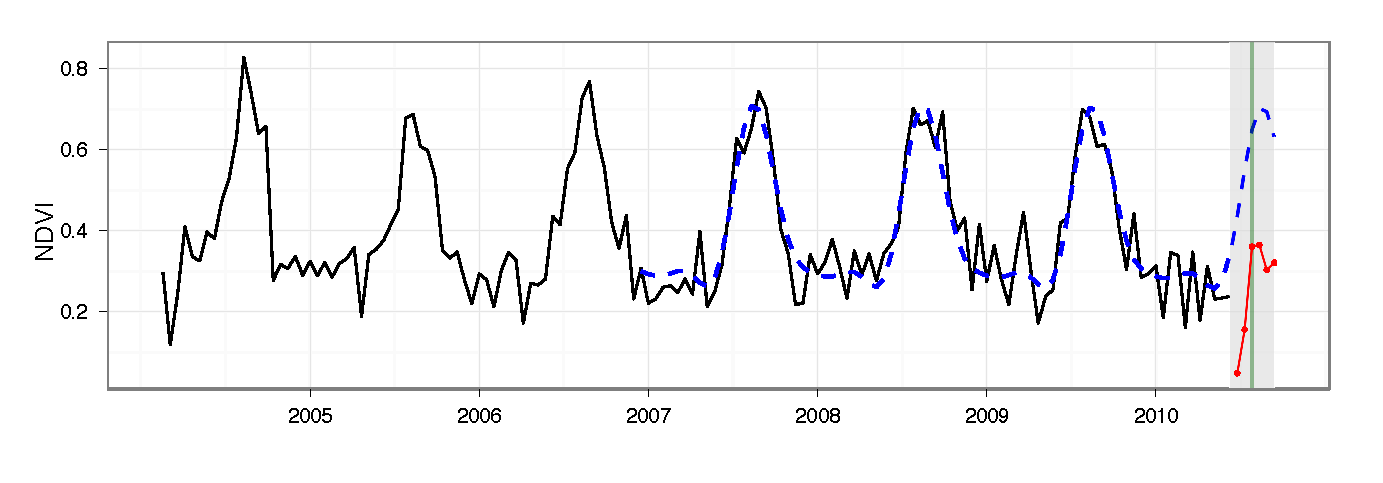
\includegraphics[width=1\textwidth]{figs/Fig1Sim_Monitoring_ggplot.eps}
  \caption{Simulated 16-day MODIS NDVI time series with $a = 0.4$, $\sigma = 0.05$, containing one simulated abrupt change with $m = -0.3$). The period from 2004 until mid 2010 (i.e., the time step just before the simulated break), is considered the \emph{history period} and the period after the simulated break is the \emph{monitoring period} (grey background). The monitoring period contains 6 observations  ($d = 6$, \textcolor{red} {red} line). The result of the monitoring approach are shown. A stable history period is identified within the history period (i.e.\ 2007 until mid 2010) and used to model and predict the normal data variation (\textcolor{blue} {blue} dashed line) to enable disturbance detection (Section~\ref{sec:MonStrucChange}).  Here, a disturbance is detected (\textcolor{OliveGreen} {green} vertical line).}
  \label{fig:SimMonitor}
\end{figure}

 \begin{figure}[htp]
\centering
    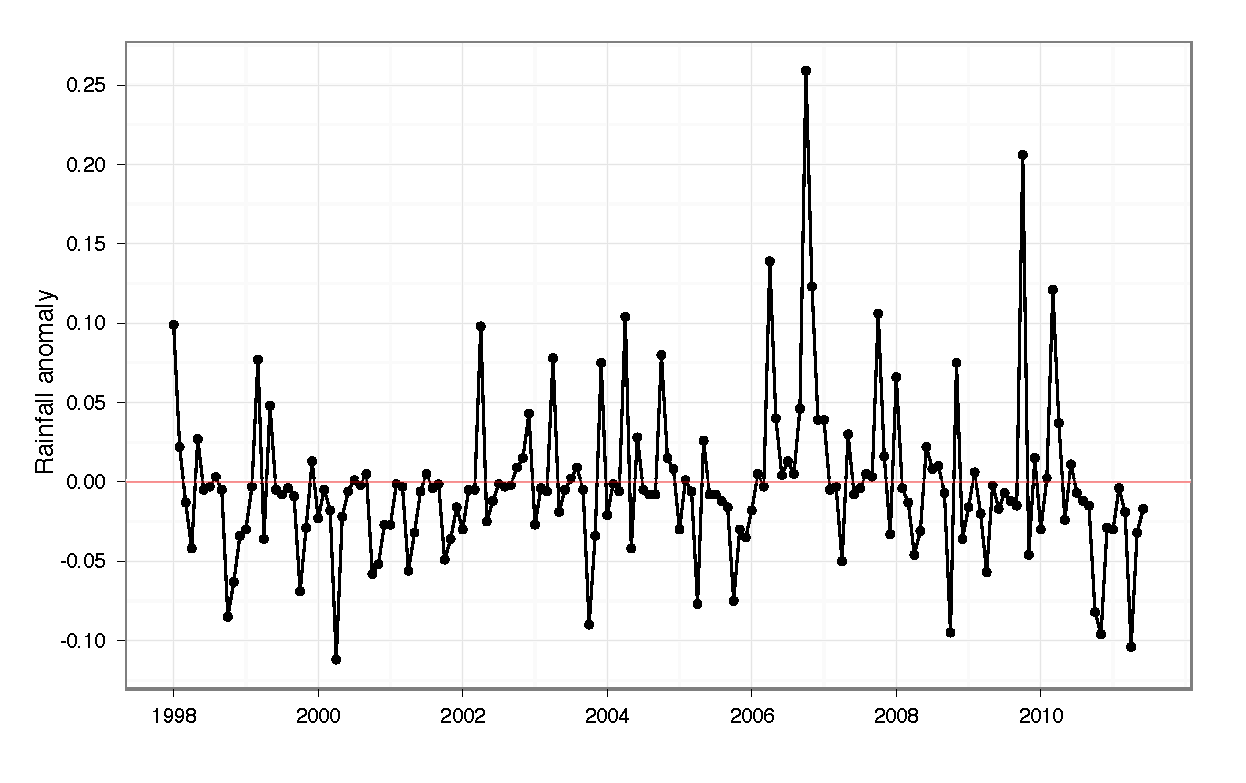
\includegraphics[width=0.8\textwidth]{figs/RainfallAnomaly.eps}
  \caption{Monthly rainfall anomalies (mm) for the period 1998--2011 measured by the tropical rainfall measuring satellite mission (TRMM) for an area in South Somalia (2\degree~Lat. and 43\degree~Long.). The time series was derived from the TRMM 3B43 climatology (version 6) data set using the online visualisation and analysis system (TOVAS). Anomalies are computed as the difference between the measured precipitation and the average climatology for the selected region \citep{Acker:2007vk}.}
  \label{fig:RF}
\end{figure}

\begin{figure} [htp]
\centering
\subfloat[][] {\label{fig:RFA} 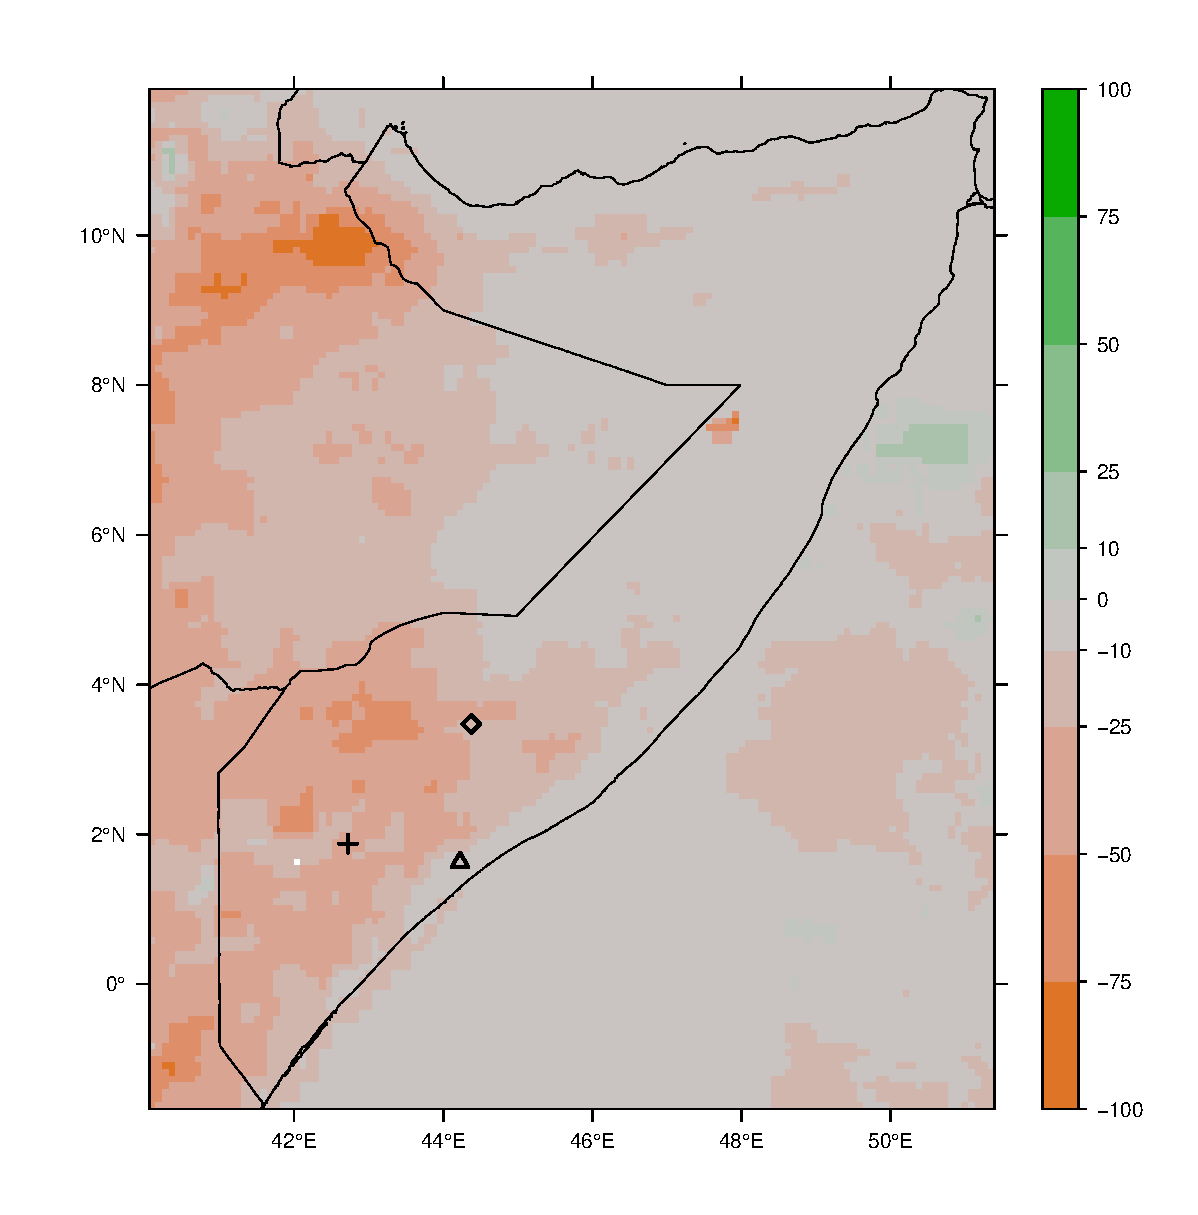
\includegraphics[height=0.55\textwidth]{figs/Rainfall_Somalia.eps} } %
 \subfloat[][] {\label{fig:LST} 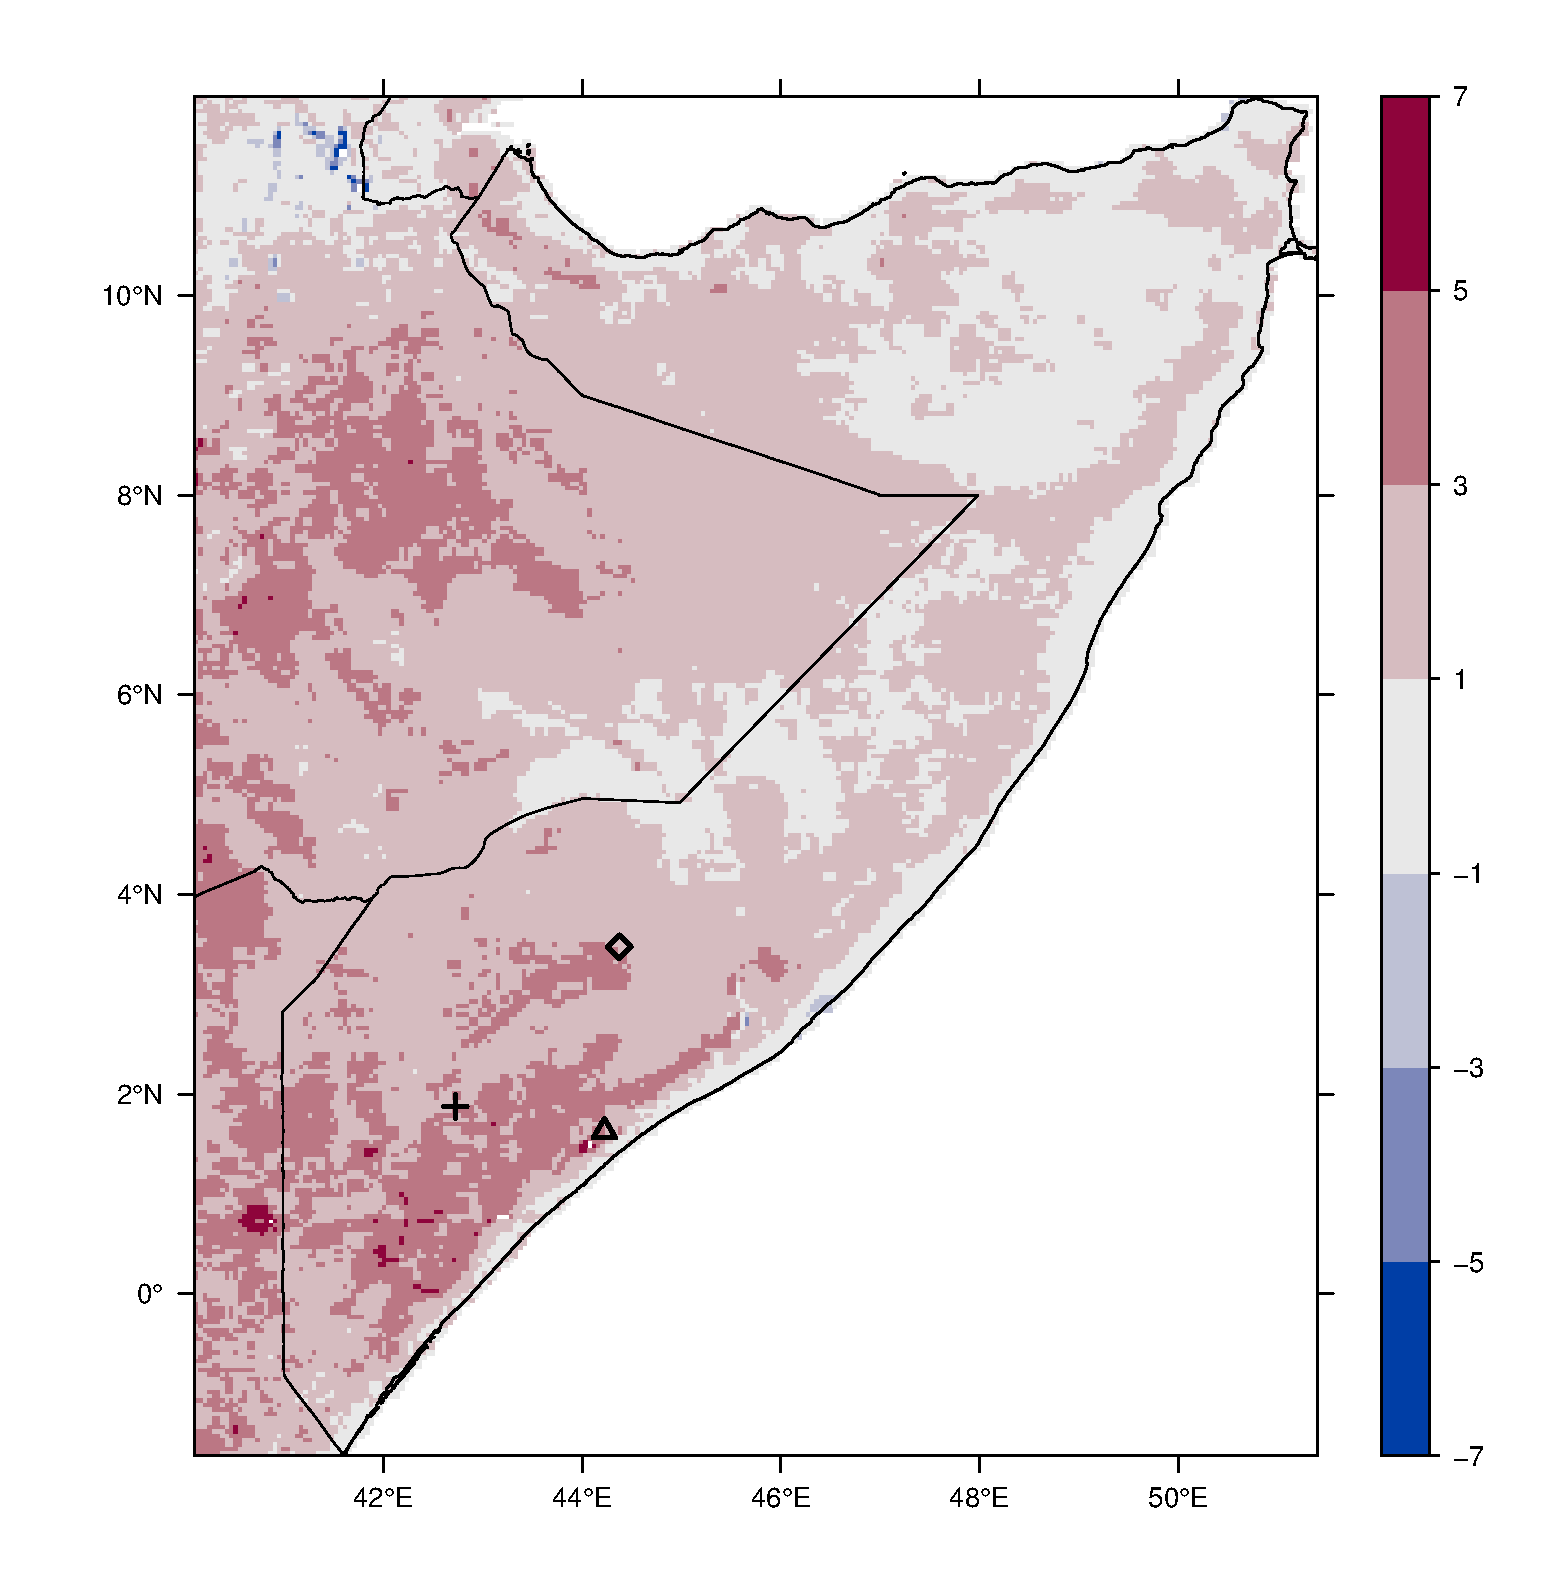
\includegraphics[width=0.55\textwidth]{figs/LSTMarchApril_Somalia.eps} } 
 \caption{Two-monthly rainfall estimates (mm, RFE2) (a)~and land surface temperature (\degree C, LST) (b)~anomaly are shown for Somalia illustrating the below normal rainfall and above normal land surface temperature during the February-March period in 2011. The RFE2 data is a merged satellite-gauge rainfall product produced by NOAA's Climate Prediction Centre at a 0.1\degree~spatial resolution. The LST product is the land surface temperature measured by the MODIS satellite and is provided at a 0.05\degree~spatial resolution. Individual observations are subtracted from the time series mean to produce anomaly data. MODIS NDVI time series (2000--2011) for three locations ($\triangle,+$~and~$\diamondsuit$) are shown in Fig.~\ref{fig:realmon}. The data were obtained using the Early Warning Explorer software tool available at \url{earlywarning.usgs.gov}. }
 \label{fig:RF_LSTSomalia}
\end{figure}

\begin{figure}[htp]
\centering
    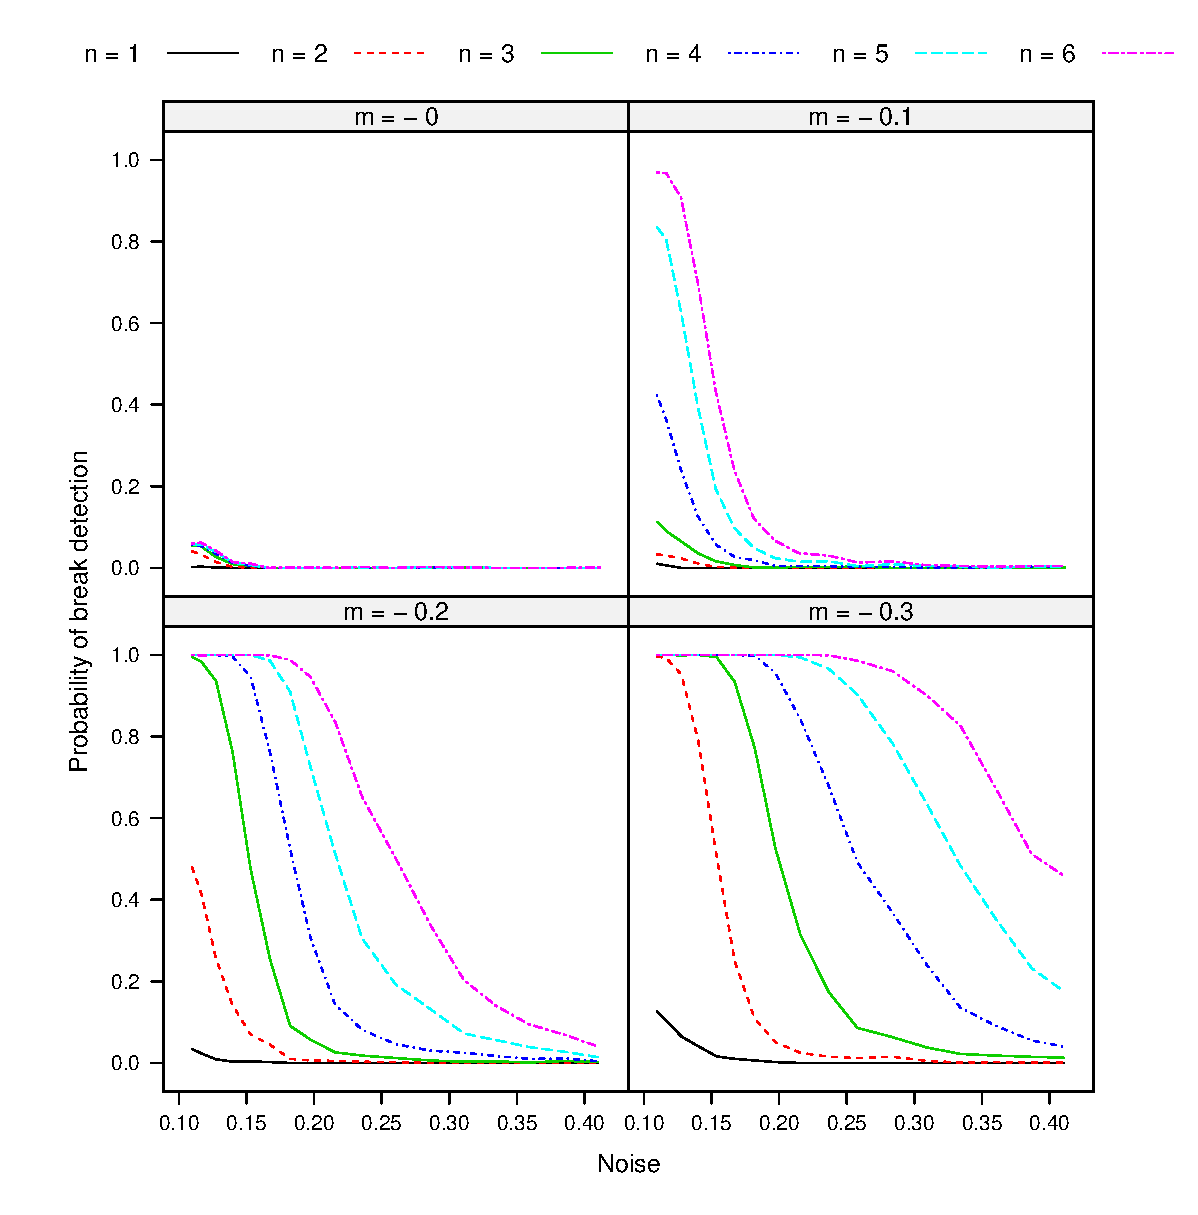
\includegraphics[height=0.9\textwidth]{figs/NrDetections_Time_1000.eps}
  \caption{Results from the simulation experiment (1000 iterations) illustrating the probability for break detection in the monitoring period while varying the amount of noise ($\sigma$), magnitude of the simulated break ($m$), and amount of data  available in the monitoring period ($d$). The units of the x and y-axis are noise (i.e., $\sigma$ NDVI of the residuals of the fitted season-trend model on the history period) and probability of detecting a break (i.e., proportion of detected breaks in 1000 iterations). See description of the simulation experiment for more details (Section~\ref{sec:Valsim}). }
  \label{fig:SimNr}
\end{figure}

\begin{figure}[htp]
\centering
% \subfloat[][] {\label{fig:spatiala} 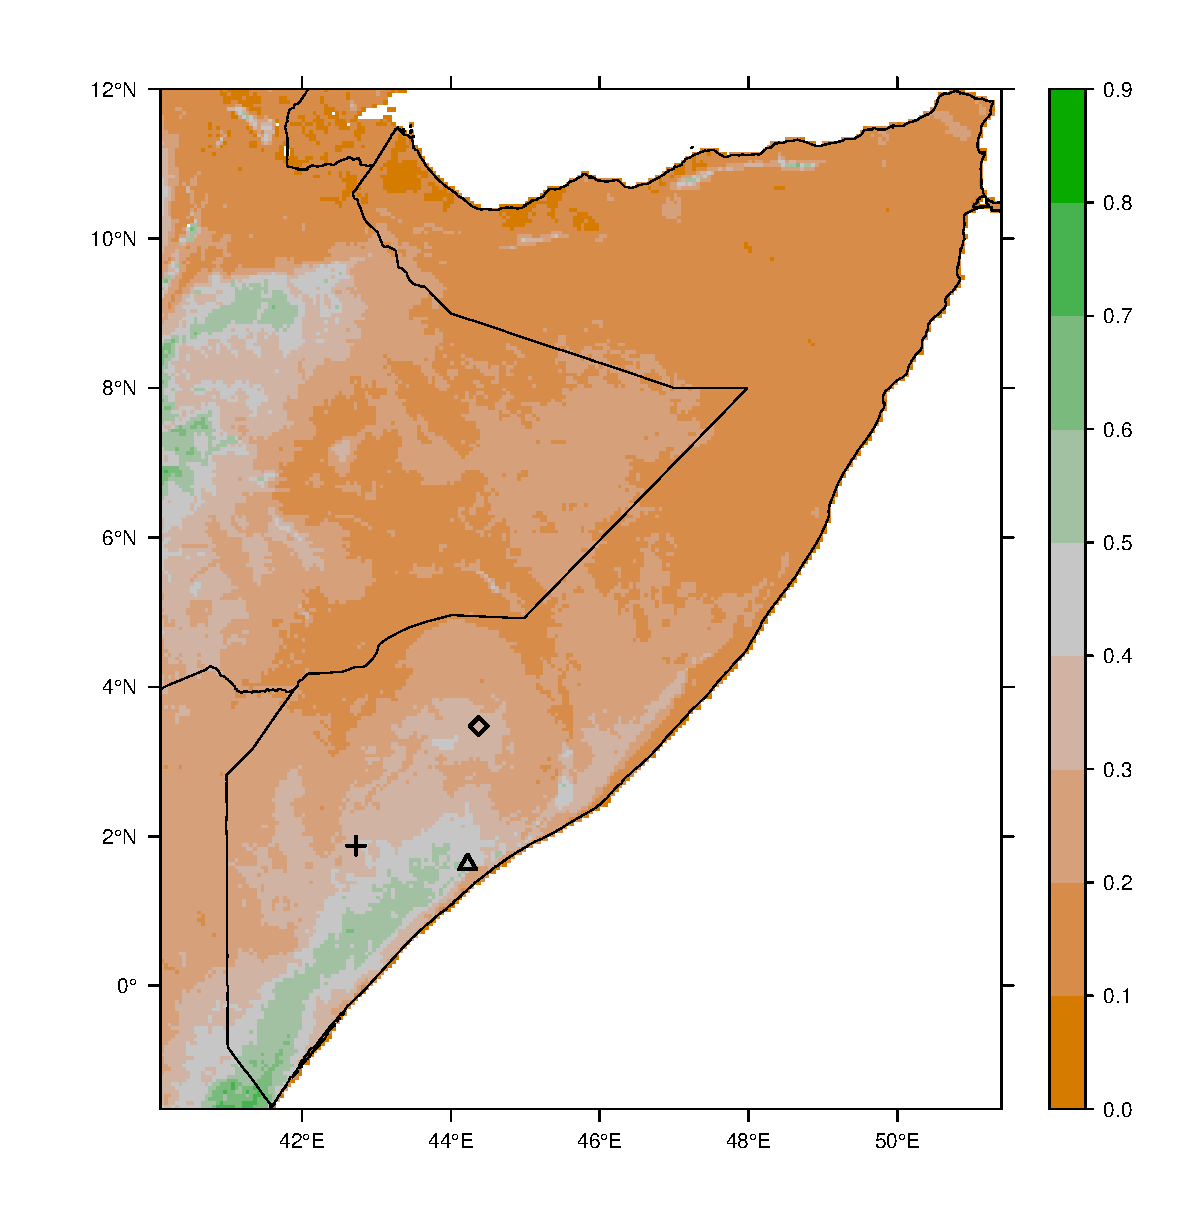
\includegraphics[height=0.55\textwidth]{figs/MedianNDVI_Somalia.eps} } %
% \subfloat[][] {\label{fig:spatialb} 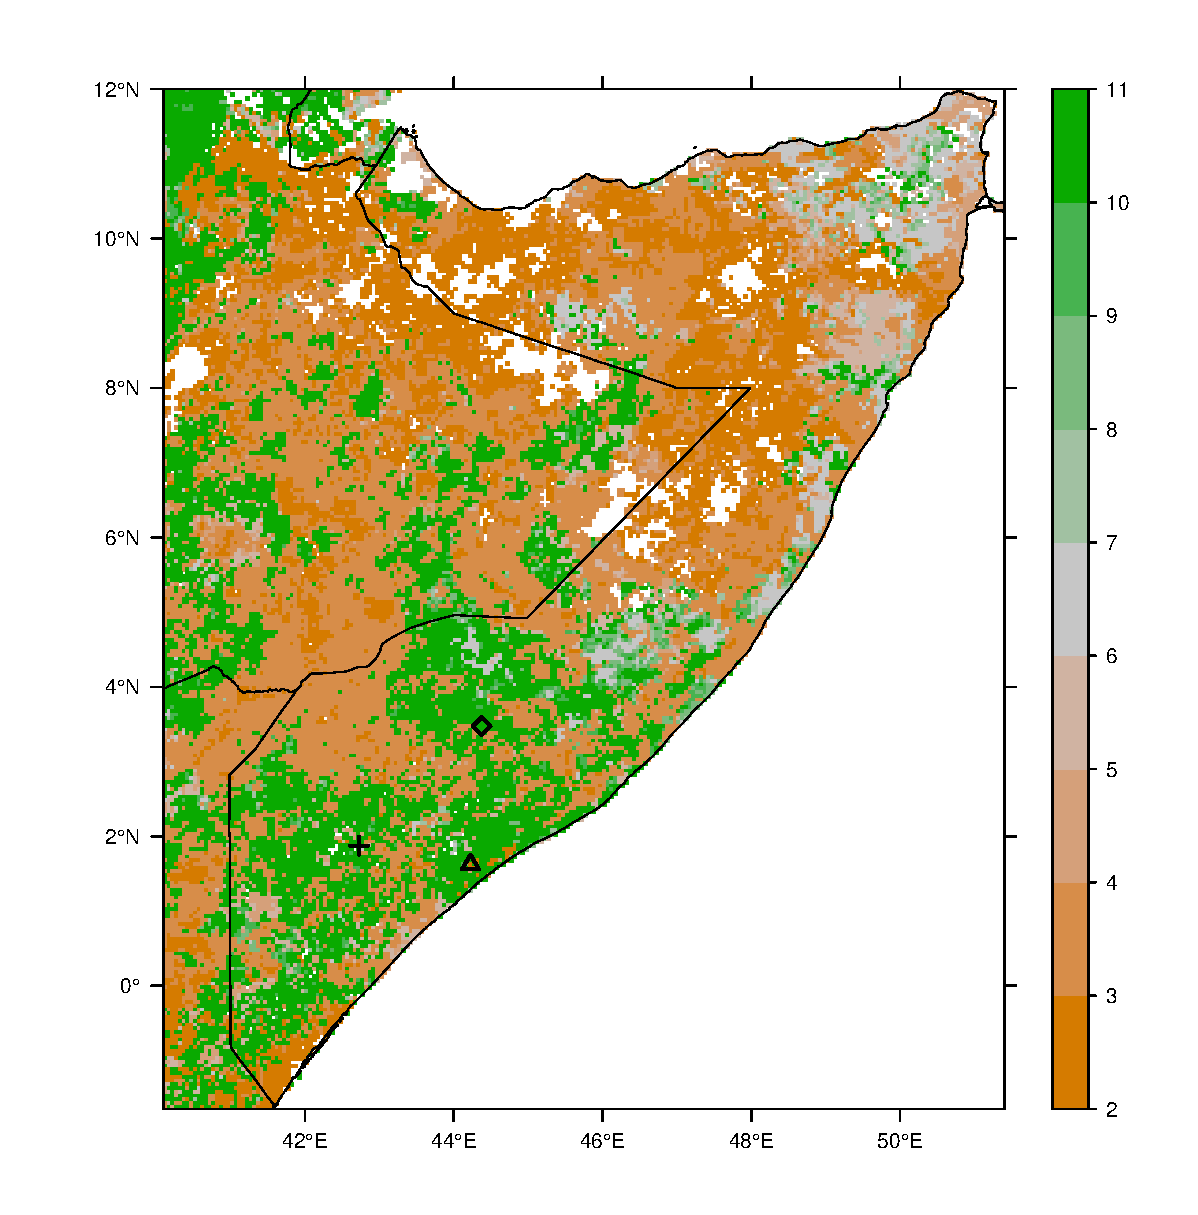
\includegraphics[width=0.55\textwidth]{figs/LengthHistoryPeriod_EA.eps} }  \\
% \subfloat[][] {\label{fig:spatialc} 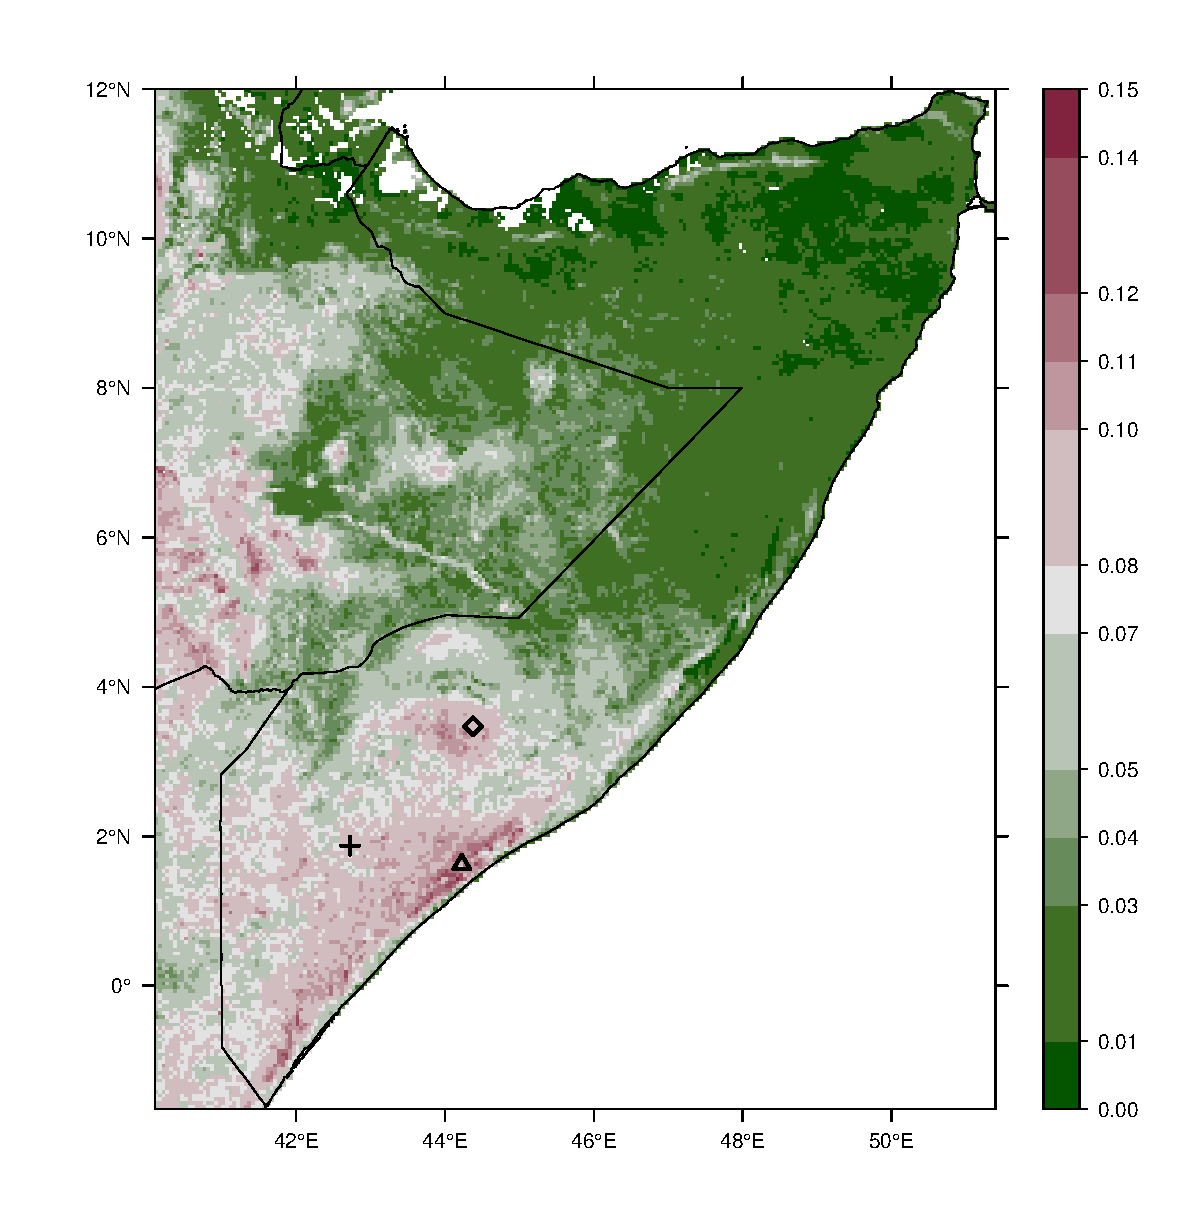
\includegraphics[width=0.55\textwidth]{figs/Noise_EA.eps} } %
%\subfloat[][] {\label{fig:spatiald} 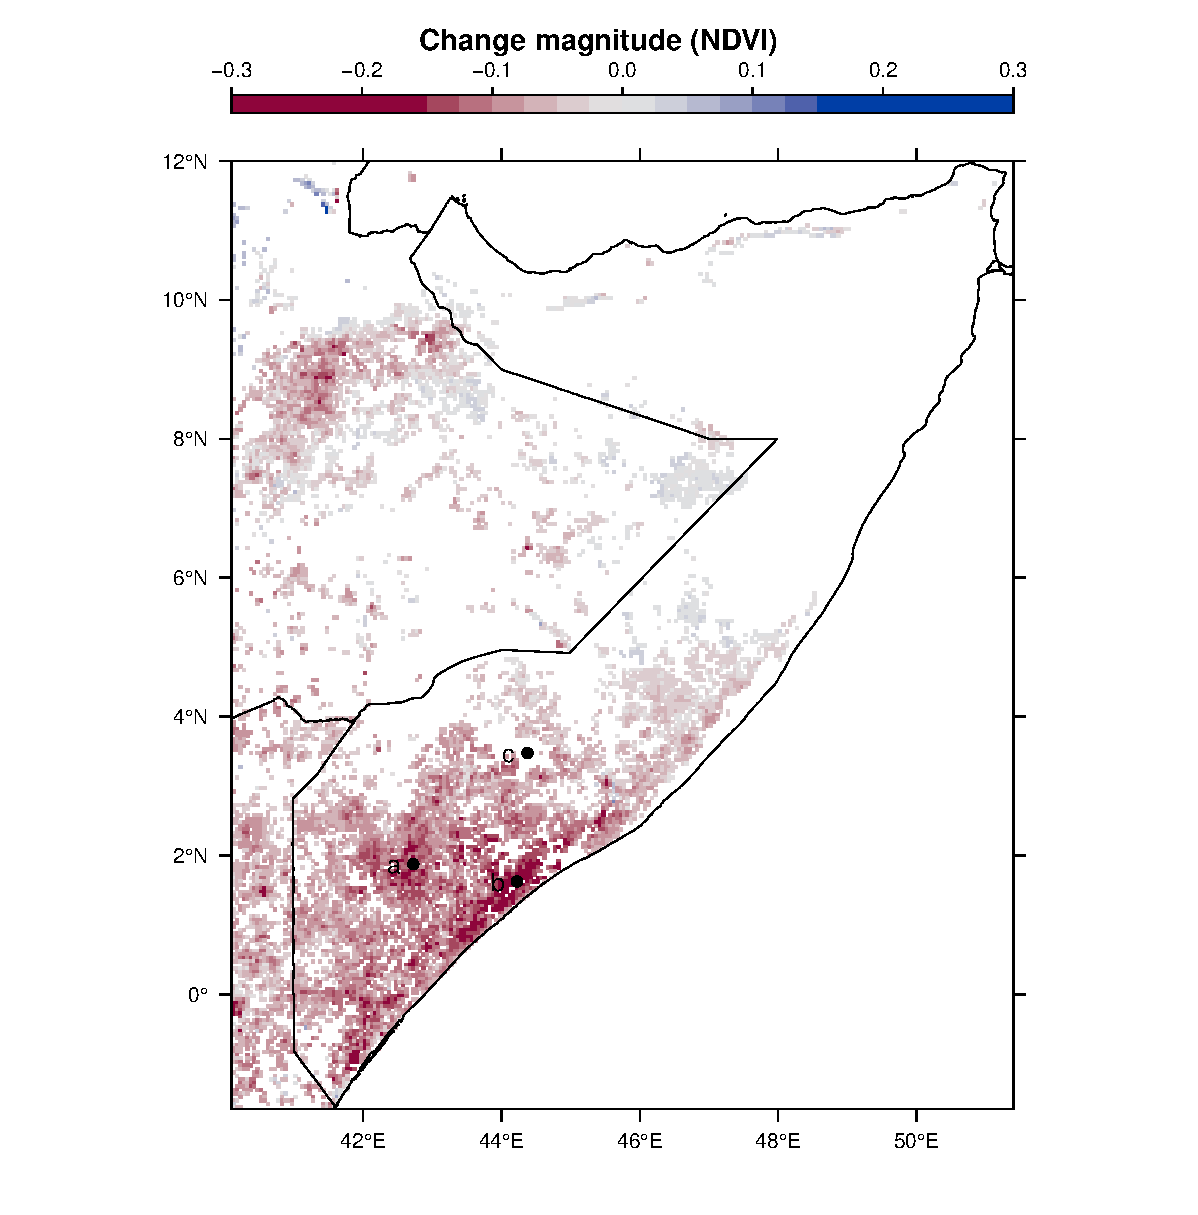
\includegraphics[width=0.55\textwidth]{figs/MagnAbnormalBreak_201012_EA.eps} }
 \caption{Results from the analysis of 16-day MODIS NDVI image time series from February 2000 until July 2011 covering Somalia; (a)~median of all NDVI
 images as a proxy for vegetation cover during the 2000--2011 period, (b)~length of the stable history period expressed in years where a shorter length is an indication of a more recent disturbance, (c)~spatial variation of the noise level (i.e.\ the standard deviation of the residuals of the stable history model), (d)~the magnitude of the detected disturbances in the monitoring period (mid 2010 onwards) where white indicates that no disturbance is detected. The analysis of~(d) was restricted to areas with minimum vegetation cover (i.e.\ median NDVI  2000--2011$> 0.2$) and length of the history period $> 2$ years. Examples for three locations ($\triangle,+$~and~$\diamondsuit$) are shown in Fig.~\ref{fig:realmon}.}
 \label{fig:spatial}
\end{figure}

\begin{figure}[htp]
\centering
    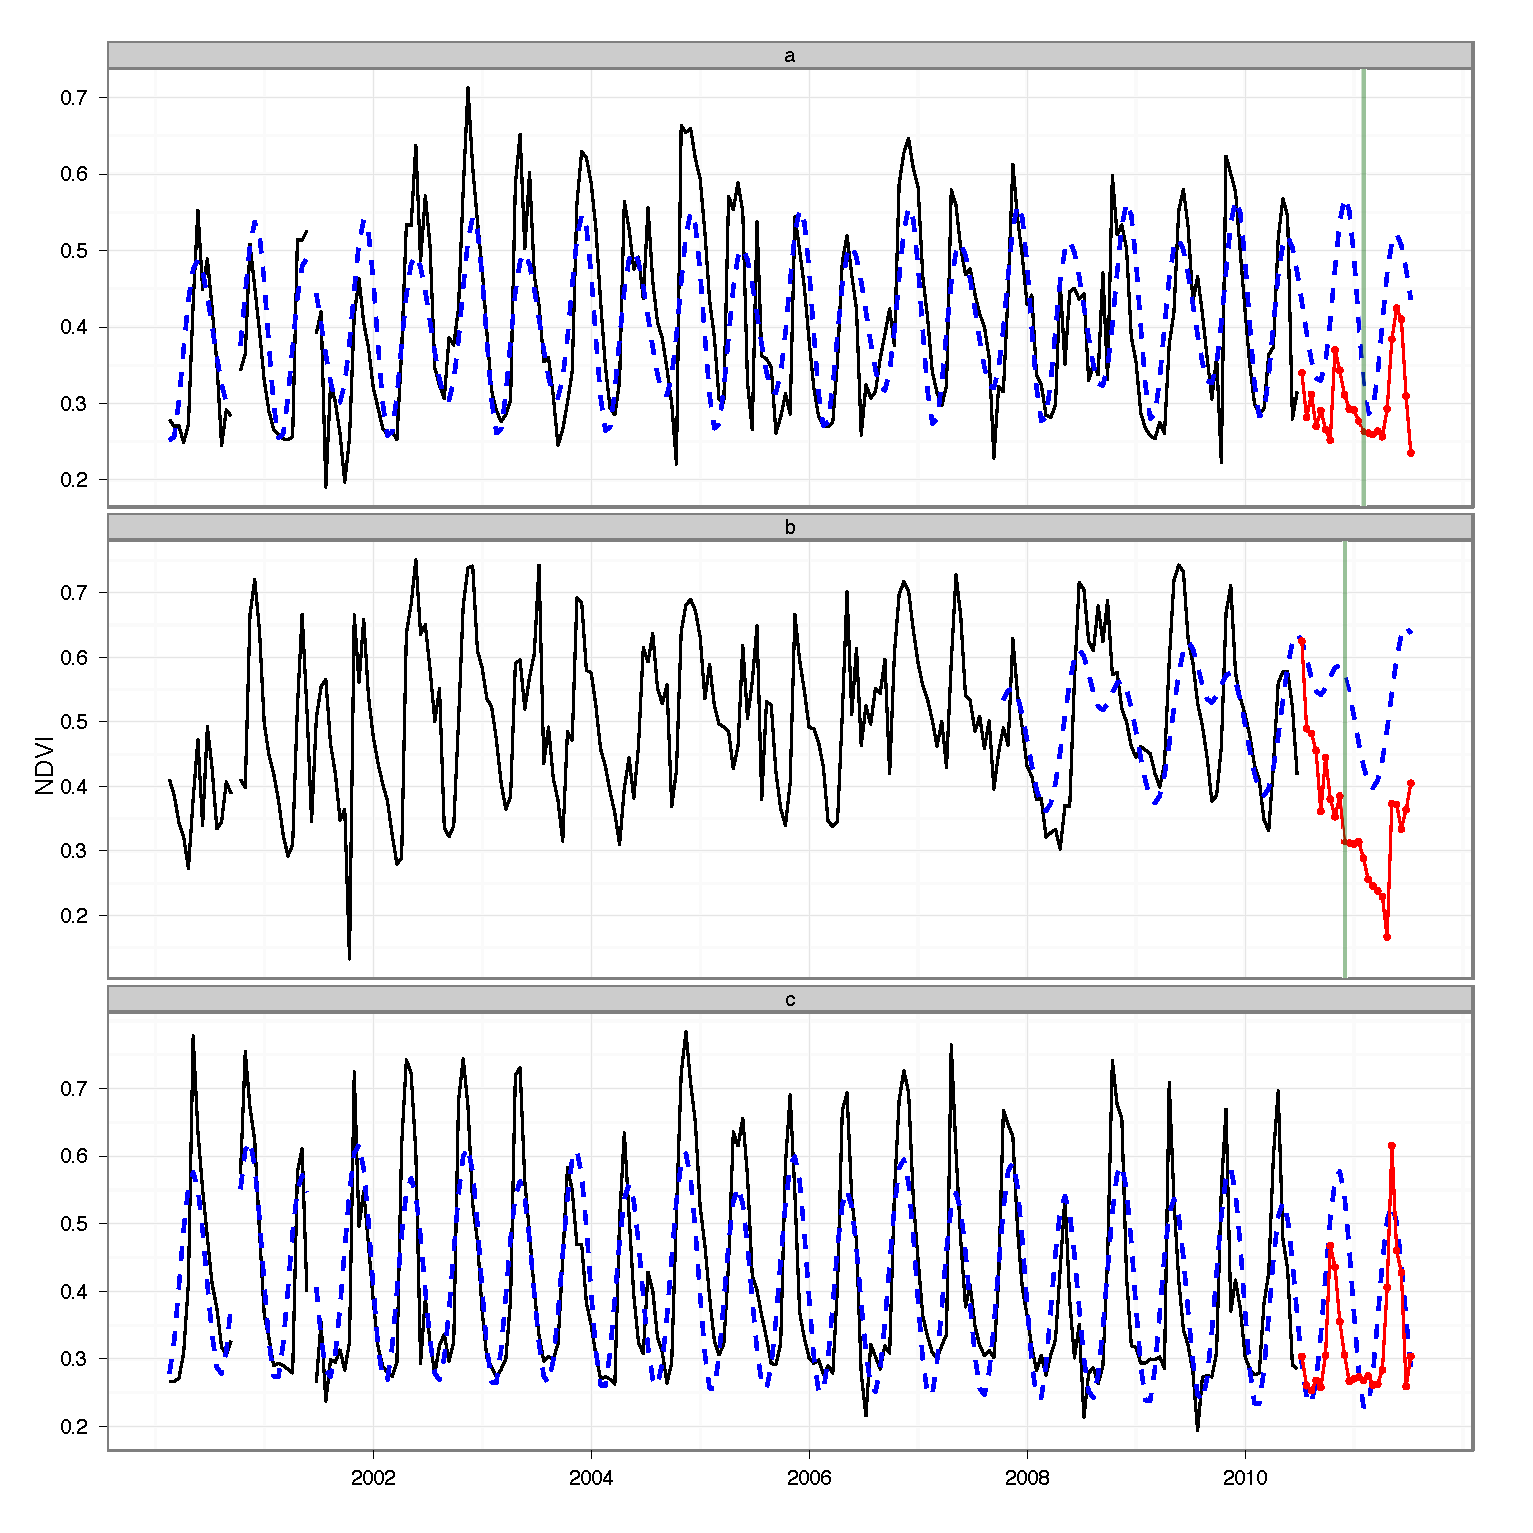
\includegraphics[width=1\textwidth]{figs/tsexampleSOM.eps}
  \caption{
 Results of real-time monitoring approach applied to 16-day MODIS NDVI time series for three locations a, b, and c, corresponding to symbols $+,~\triangle$~and~$\diamondsuit$ shown in Fig.~\ref{fig:spatial}. The period from 2000 until mid 2010, is considered the \emph{history period} and the period from 2010 onwards is the \emph{monitoring period} (grey background, \textcolor{red} {red} line). The stable history period within the history period (\textcolor{blue} {blue} dashed line) is used to model and predict the normal data variation and enable disturbance detection in the monitoring period (Section~\ref{sec:MonStrucChange}).  A disturbance is detected (\textcolor{OliveGreen} {green} line) in Fig~\ref{fig:realmon}a and~\ref{fig:realmon}b.}
  \label{fig:realmon}
\end{figure}
 
% In both time series a break (vertical red dashed line in 2006) is detected in the monitoring period (i.e., 2006) while using 2000 until end of 2005 as a history period. A stable history period (blue dots) is automatically detected with the history period. The method is able to deal with time series with data gaps (e.g., after cloud removal) which is illustrated by data gaps within the data analysed and model fit based on the stable history period.


\end{document}

